\documentclass[]{article}
\usepackage{amsmath}
\usepackage{graphicx}
\usepackage{caption}
\graphicspath{{C:\Users\Vale\Dropbox\Poli\Erasmus\KTH\Statitical Methods for Applied Computer Science\DD2447_2017}}

% Title Page
\title{Statistical Methods in \\ Applied Computer Science, Fall 2017 \\ Assignment 2}
\author{Valeria Callioni, Viran Ribic - \\ Assignment 2 Group 3}


\begin{document}
\maketitle

\newpage

\section*{2.1 SMC for the stochastic volatility model}
In this first task we have to consider the stochastic volatility model
\begin{align*}
	X_t|X_{t-1} = x_{t-1} \sim \mathcal{N}(x_t | \phi x_{t-1},\sigma^2), && t=1...T 
	\\
	Y_t|X_t = x_t \sim \mathcal{N}(y_t | 0, \beta^2e^{x_t}), && t=1...T 
\end{align*}
where we assume stationarity by setting 
$$
X_0 \sim \mathcal{N}(x_0 | 0, \frac{\sigma^2}{1-\phi^2})
$$
The latent variable $X_t$ denotes the underlying volatility, i.e. the variations in the price of some financial asset, and $Y_t$ denotes the observed scaled log-returns from the asset. 
First we generate parameters together with a synthetic data vector $y_{1:T}$, $T = 500$, based on the stochastic volatility model, using the generator provided; then we implement a SMC algorithm with and without resampling with the final goal of estimating the likelihood for different values of the parameter $\beta$, considering the other parameters to be known. 

Let us explain the setting. $\{X_t\}_{t\geq0}$ is a discrete-time Markov process such that 
$$
X_0 \sim \mu(x_0) \text{ and } X_t|X_{t-1} = x_{t-1} \sim f(x_t|x_{t-1})
$$
We are interested in estimating $\{X_t\}_{t\geq0}$ but only have access to the values of the process $\{Y_t\}_{t\geq1}$. We assume that, given $\{X_t\}_{t\geq0}$, the observations $\{Y_t\}_{t\geq1}$ are statistically independent and their marginal densities are given by
$$
Y_t|X_t = x_t \sim g(y_t|x_t).
$$
We also assume that the transition and observation densities are independent of the time index $n$. This leads to a Bayesian model with the prior distribution given by 
$$
p(x_{0:T}) = \mu(x_0)\prod_{t=1}^{T}f(x_t|x_{t-1})
$$
and the likelihood
$$
p(y_{1:T}|x_{0:T}) = \prod_{t=1}^{T}g(y_t|x_t).
$$
Then the posterior distribution is
$$
p(x_{0:T}|y_{1:T}) = \frac{p(x_{0:T},y_{1:T})}{p(y_{1:T})}.
$$
Since our final goal is to determine the log-likelihood of the data for different values of the parameter $\beta$, we want to approximate $p(y_1)$ at the first time instance, $p(y_{1:2})$ at the second time instance and so on.

We want to use SMC methods, a general class of Monte Carlo methods that sample senquentially from a sequence of target probability densities $\{ \pi_t(x_{1:t}) \}$ of increasing dimension. In particular, 
$$
\pi_t(x_{0:t}) = \frac{\gamma_t(x_{0:t})}{Z_t}
$$
where 
$\gamma_t$ is known pointwise and the normalizing constant $Z_t$ is known.

In our particular case, that can be consideres as a Filtering problem, we have
$$
\gamma_t(x_{1:t}) = p(x_{0:T},y_{1:T})
$$ 
that means
$$
\pi_t(x_{0:t}) = p(x_{0:T}|y_{1:T}) \text{ and } Z_t = p(y_{1:t}).
$$
Then, the proposal distibution is given by 
$$
q_t(x_t|x_{0:t-1}) = q_t(x_t|y_t, x_{t-1})
$$
that leads to incremental weights of the form
$$
\alpha_t(x_{0:t}) = \alpha_t(x_{t-1:t}) = \frac{g(y_t|x_t)f(x_t|x_{t-1})}{q_t(x_t|y_t, x_{t-1})}.  
$$
In our setting, the conditional prior can be employed as a proposal distribution. Then, the incremental weights are simply given by
$$
\alpha_t(X_{t-1:t}^i) = g(y_t|X_t^i).
$$
To obtain the log-likelihood, at each iteration we have to compute
\begin{align*}
	\log\hat{p}(y_{1:t}) = & \log[ \hat{p}(y_1) \prod_{k=2}^{t} p(y_k|y_{1:k-1})] \\
	= & \log \hat{p}(y_1) + \sum_{k=2}^{t} \log p(y_k|y_{1:k-1})
\end{align*}
where
\begin{align*}
	\hat{p}(y_1) = & \sum_{i=1}^{N} p(y_1|X_1^i)p(X_1^i) \\
	= & \sum_{i=1}^{N} p(y_1|X_1^i)[\sum_{j=1}^{N}p(X_1^i|X_0^j)p(X_0^j)] \\
	= & \sum_{i=1}^{N} g(y_1|X_1^i)[\sum_{j=1}^{N}f(X_1^i|X_0^j)\mu(X_0^j)]
\end{align*}
and
$$
\hat{p}(y_t|y_{1:t-1}) = \sum_{i=1}^{N}W_{n-1}^i\alpha_t(X_{t-1:t}^i).
$$
\subsection*{Question 1}
Following this reasoning, we implemented the SMC algorithm. The first step is given by the initialization, that is 
\begin{enumerate}
	\item[-] sample $X_0^i \sim \mathcal{N}(0, \frac{\sigma^2}{1-\phi^2})$
	\item[-] sample $X_1^i \sim \mathcal{N}(\phi x_0^i,\sigma^2) $ 
	\item[-] compute the weights $w_1(X_1^i) = \sum_{j=1}^{N}f(X_1^i|X_0^j)\mu(X_0^j)$ and the normalized weights $W_1(X_1^i)$
	\item[-] compute the incremental weights $ \alpha_1(X_1^i) = g(y_1|X_1^i)w_1(X_1^i) $
	\item[-] compute $\log \hat{p}(y_1)$ as previously stated. 
\end{enumerate}
Then, at each iteration $t \geq 2$:
\begin{enumerate}
	\item[-] sample $X_t^i \sim \mathcal{N}(\phi x_{t-1}^i,\sigma^2) $
	\item[-] compute the incremental weights $ \alpha_t(X_{t-1:t}^i) = g(y_t|X_t^i) $
	\item[-] compute $\log \hat{p}(y_t|y_{1:t-1})=\log\sum_{i=1}^{N}W_{t-1}^i\alpha_t(X_{t-1:t}^i)$
	\item[-] compute the weights $
	w_t(X_{0:t}^i)=w_0(X_1^i)\prod_{k=2}^{t}\alpha_k(X_{0:k}^i)$ and the normalized weights
\end{enumerate}
Considering a coarse grid for $\beta$, given by 20 points equally-spaced in the interval $(0,2)$ and running 10 times the SMC for every value of $\beta$, we obtained the following result:
\begin{figure}
	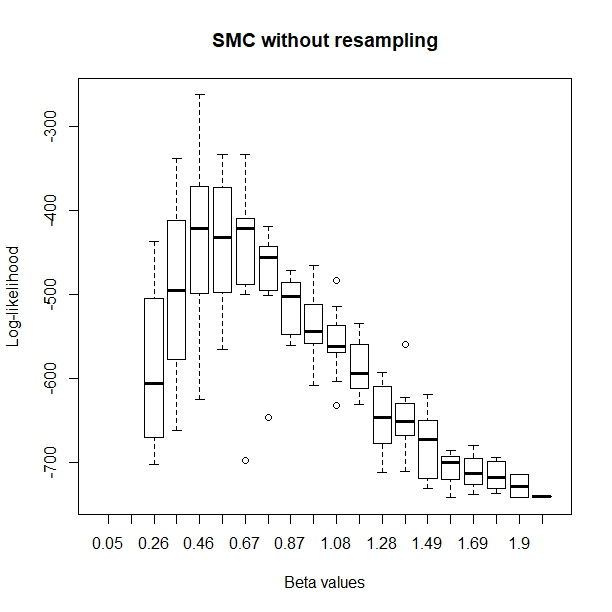
\includegraphics[width=\columnwidth]{task1/SIS_N_100_T_500.jpeg}
	\caption{Log-likelihood running SIS 10 times, with $N=100$ and $T=500$}
\end{figure}
where we can see that the maximum value of the log-likelihood is reached, in mean, for $\beta=0.46$.

\subsection*{Question 2}
Introducing resampling means to sample from an approximation $\hat{\pi}(x_{1:t})$ which was itself obtained by sampling. We resample $N$ times from $\hat{\pi}(x_{1:t})$, which is equivalent to associating a number of offspring $N_t^i$ with each particle $X_{1:t}^i$ in such a way that $N_t^{1:N} = (N_t^1, ..., N_t^N)$ follow a multinomial distribution with parameter vector $(N, W_t^{1:N})$ and associating a weight of $\frac{1}{N}$ with each offspring. Since we use systematic resampling, the previous algorithm becomes as follows:

Initialization:
\begin{enumerate}
	\item[-] sample $X_0^i \sim \mathcal{N}(0, \frac{\sigma^2}{1-\phi^2})$
	\item[-] sample $X_1^i \sim \mathcal{N}(\phi x_0^i,\sigma^2) $ 
	\item[-] compute the weights $w_1(X_1^i) = \sum_{j=1}^{N}f(X_1^i|X_0^j)\mu(X_0^j)$ and the normalized weights $W_1(X_1^i)$
	\item[-] compute the incremental weights $ \alpha_1(X_1^i) = g(y_1|X_1^i)w_1(X_1^i) $
	\item[-] sample $U_1 \sim \mathcal{U}[0, \frac{1}{N}]$ and define $U_i = U_1 + \frac{i-1}{N}$
	\item[-] set $N_1^i = |\{ U_j: \sum_{k=1}^{i-1}W_1^k \leq U_j \leq \sum_{k=1}^{i}W_1^k \}|$ with the convention $\sum_{k=1}^{0}=0$, and set the particles to be $N$ equally-weighted of the form $\{\frac{1}{N}, X_1^i\}$
	\item[-] update the values of the incremental weights  $ \alpha_1(X_1^i) $ given the new equally-weighted particles
	\item[-] compute $\log \hat{p}(y_1)$. 
\end{enumerate}
Then, at each iteration $t \geq 2$:
\begin{enumerate}
	\item[-] sample $X_t^i \sim \mathcal{N}(\phi x_{t-1}^i,\sigma^2) $
	\item[-] compute the incremental weights $ \alpha_t(X_{t-1:t}^i) = g(y_t|X_t^i) $
	\item[-] sample $U_1 \sim \mathcal{U}[0, \frac{1}{N}]$ and define $U_i = U_1 + \frac{i-1}{N}$
	\item[-] set $N_t^i = |\{ U_j: \sum_{k=1}^{i-1}W_t^k \leq U_j \leq \sum_{k=1}^{i}W_t^k \}|$ with the convention $\sum_{k=1}^{0}=0$, and set the particles to be $N$ equally-weighted of the form $\{\frac{1}{N}, X_t^i\}$
	\item[-] update the values of the incremental weights  $ \alpha_t(X_{t-1:t}^i) $ given the new equally-weighted particles
	\item[-] compute $\log \hat{p}(y_t|y_{1:t-1})=\log\sum_{i=1}^{N}\frac{1}{N}\alpha_t(X_{t-1:t}^i)$
	\item[-] compute the weights $
	w_t(X_{0:t}^i)=w_0(X_1^i)\prod_{k=2}^{t}\alpha_k(X_{0:k}^i)$ and the normalized weights
\end{enumerate}
Considering the same coarse grid for $\beta$ as before, and running 10 times the SMC with resampling for every value of $\beta$, we obtained the following result:
\begin{figure}
	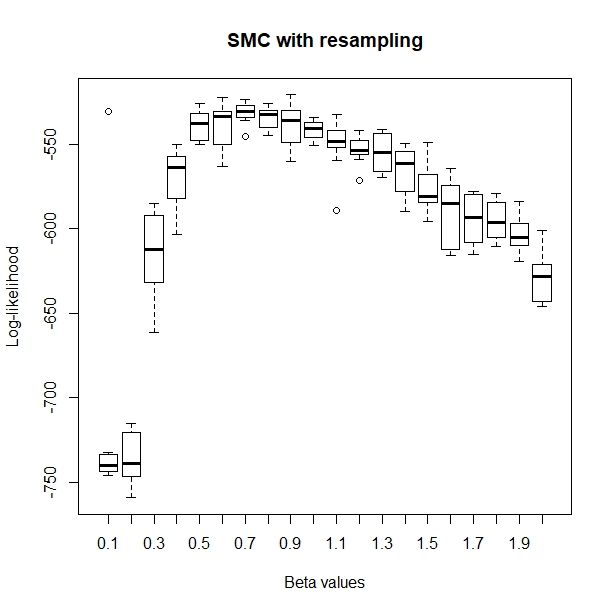
\includegraphics[width=\columnwidth]{task1/SIR_N_100_T_500.jpeg}
	\caption{Log-likelihood running SIR 10 times, with $N=100$ and $T=500$}
\end{figure}
where we can see that the maximum value of the log-likelihood is reached, in mean, for $\beta=0.357$.

In both experiments we considered $N=100 \text{ and } T=500$. We can observe that the variance of the estimator decreases using resampling. 

\subsection*{Question 4}
Finally, we run the algorithm with different values of $N$ and $T$, to study how these parameters affect the variance in the log-likelihood estimate. 

\begin{figure}
	\begin{center}
		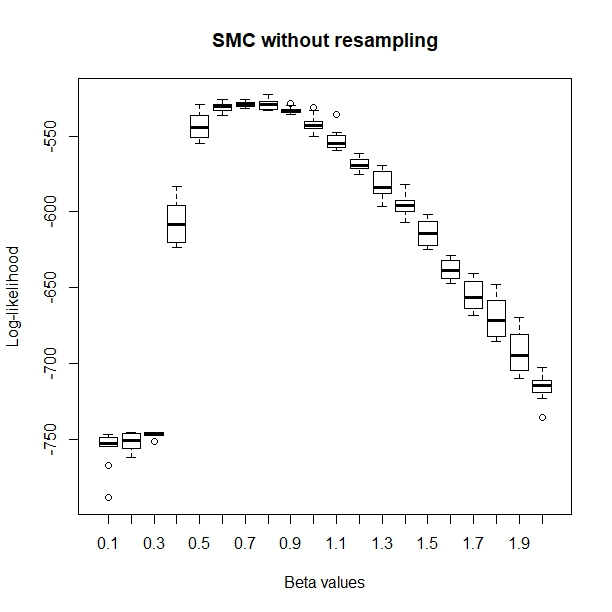
\includegraphics[width=.4\textwidth]{task1/SIS_N_1000_T_500.jpeg}
		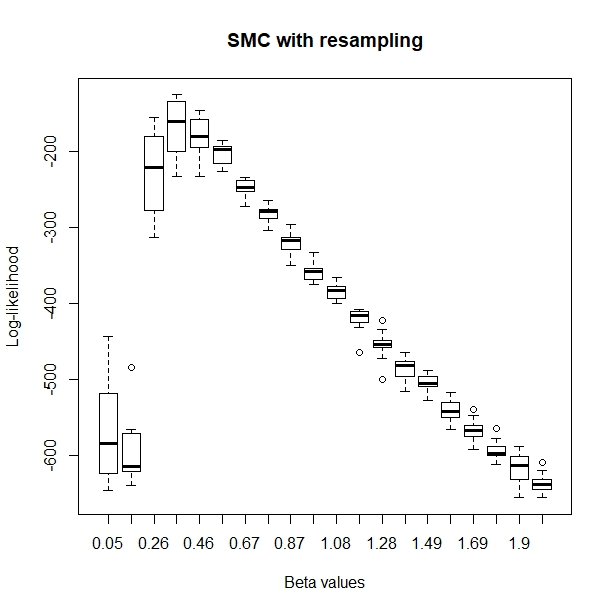
\includegraphics[width=.4\textwidth]{task1/SIR_N_1000_T_500.jpeg}
		\caption*{$N=1000$ and $T=500$}
		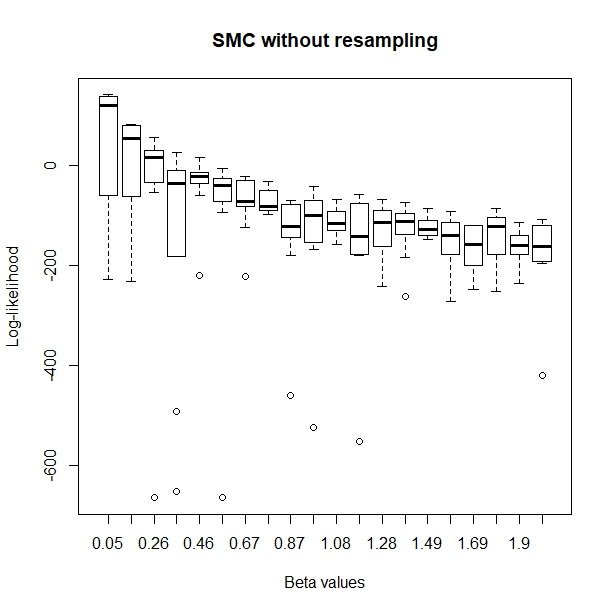
\includegraphics[width=.4\textwidth]{task1/SIS_N_100_T_100.jpeg}
		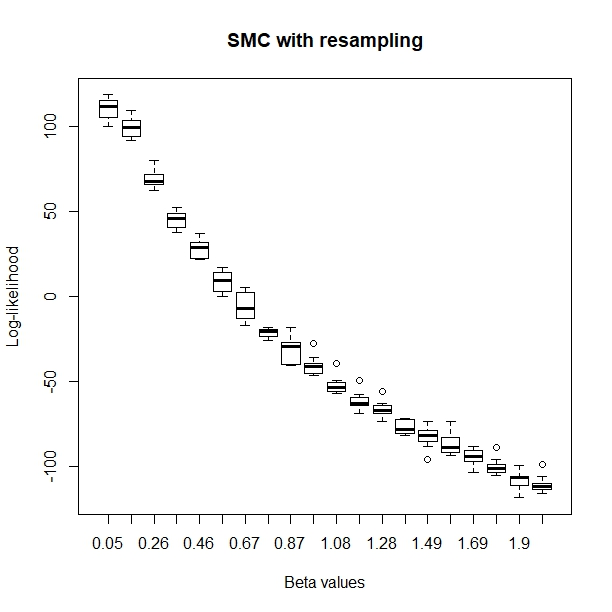
\includegraphics[width=.4\textwidth]{task1/SIR_N_100_T_100.jpeg}
		\caption*{$N=100$ and $T=100$}
		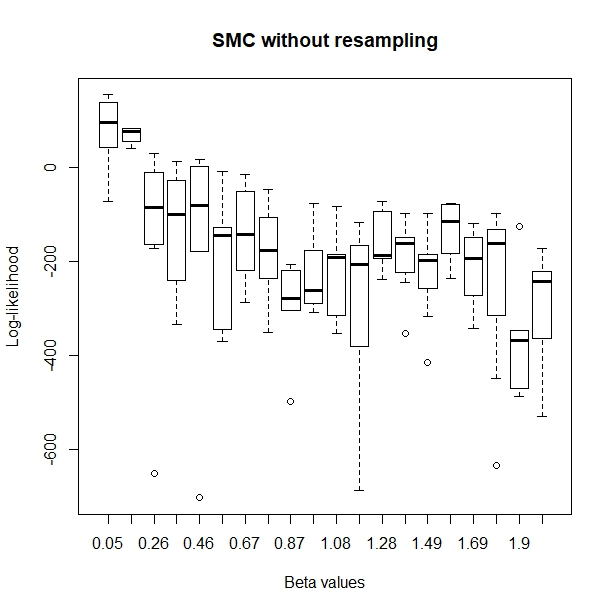
\includegraphics[width=.4\textwidth]{task1/SIS_N_1000_T_100.jpeg}
		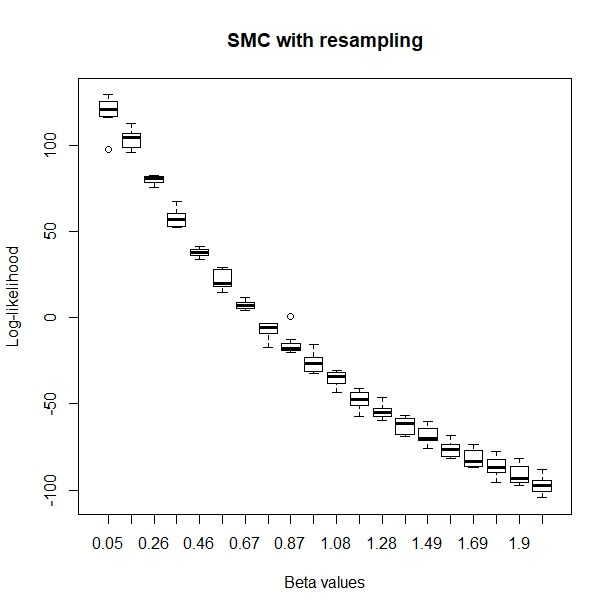
\includegraphics[width=.4\textwidth]{task1/SIR_N_1000_T_100.jpeg}
		\caption*{$N=1000$ and $T=100$}
	\end{center}
	\caption{Comparison of the results for different values of $T$ and $N$}
\end{figure}

From Figure 3, we observe that for smaller values of T we have a correct estimation of the true value of $\beta$ (i.e., the log-likelihood is maximized for the true value of $\beta$), that is 0.1011. This is due to the fact that for large values of $T$ the particle filtering may degenerate. But, in any case, the SIR algorithm performs better than the SIS one, as we expect. 

\newpage

\section*{2.3 MCMC for the train}
We are given a problem that models a railway with a single train. The map of the tracks is represented by an undirected graph $G=(V,E)$, such that each node has degree 3 and at each vertex edges are labeled $0, L or R$. Each vertex represents a switch: if the train comes from the direction of $L$ or $R$, it always leaves in the direction 0; if the train comes from the direction $0$, it will leave in either direction $L$ or $R$, depending on the state of the switch. The switch has prior probability 1/2 for each direction, but will remain the same throughout the train run. A switch setting is a function $\alpha : V(G) \rightarrow \{L,R\}$

We observe a sequence of $T$ signals, each one representing the label of the edge through which the train has exited a vertex. But the sensors are noisy, and with probability $p = 0.05$, the train reports a random other signal than real direction in which it passed the switch. 

We are given a DP algorithm to compute $p(s,O|G,\alpha)$, where $s=(v,e)$ is called stop position; and the final goal is to estimate the probability distribution of the vector $\alpha(\mathbf{v}) = (\alpha(v_1), ..., \alpha(v_N))$,  where $ N=|V(G)| $, using MCMC.

\subsection*{Question 8}
We implemented the class $Graph$ to generate the map of the railway. This class has the following attributes:
\begin{enumerate}
	\item[-] $V$, the number of nodes 
	\item[-] the degree of the graph ($degree=3$ in our setting) 
	\item[-] $A$, the adjacency matrix, where $A_{ij}=1$ if edge $(i,j)$ exists and $A_{ij}=0$ otherwise
	\item[-] $G$, the matrix representing the labels of the edges, where $G_{ij} \ \in \ \{ 0,1,2,3\} $. We used the convention that 0 represents 0, 1 represents $L$, 2 represents $R$ and 3 is assigned to edges that do not exist.
\end{enumerate} 
The map is created randomly, being sure that each vertex has degree 3 and assigning the 3 different labels to the existing edges.

The class $Train$ actually represents our setting: it has a graph, the map; the vector of obervations $O$ and the associated $path$. Observations are generated randomly and, in the end, some noise is added.

In the MCMC Metropolis Hastings algorithm that we propose, states are switch settings vectors and, at each step, the algorithm performs the following operations:
\begin{enumerate}
	\item[-] propose a new switch setting vector, by simply picking a random vertex and changing its setting. The candidate new state is chosen in this way since we have no particular assumptions and we decided to consider a uniform proposal distribution;
	\item[-] accept the new switch setting with acceptance probability 
	$$
	r(\mathbf{\alpha}_{new}|\mathbf{\alpha}_{old}) = min\{1, a(\mathbf{\alpha}_{new}|\mathbf{\alpha}_{old})\},
	$$
	where
	$$
	a(\mathbf{\alpha}_{new}|\mathbf{\alpha}_{old}) = \frac{p^*(\mathbf{\alpha}_{new})}{p^*(\mathbf{\alpha}_{old})}\frac{q(\mathbf{\alpha}_{old}|\mathbf{\alpha}_{new})}{q(\mathbf{\alpha}_{new}|\mathbf{\alpha}_{old})} 
	$$
	where $p^*$ is the target distribution and $q$ is the proposal distribution, which we assume to be symmetric. So,
	$$
	a(\mathbf{\alpha}_{new}|\mathbf{\alpha}_{old}) = \frac{p(D|\mathbf{\alpha}_{new})}{p(D|\mathbf{\alpha}_{old})} \frac{p(\mathbf{\alpha}_{new})}{p(\mathbf{\alpha}_{old})}
	$$
	Since we have uniform prior for the switch setting of each node and we assume switch settings of different nodes to be independent, and since our data $D$ are given by the vector of observations $\mathbf{O}$ we have
	$$
	a(\mathbf{\alpha}_{new}|\mathbf{\alpha}_{old}) = \frac{p(\mathbf{O}|G,\mathbf{\alpha}_{new})}{p(\mathbf{O}|G,\mathbf{\alpha}_{old})}
	$$
	The probability $p(\mathbf{O}|G,\mathbf{\alpha})$ can be computed using the DP algorithm provided, since it suffices to sum over the all possible stop positions, given particular switch settings. 
\end{enumerate}
At the end we obtain sample switch settings, that we store just after the $burn-in$ phase, and their associated probability.

\subsection*{Question 9}
To run the program, we set $V=6$ and $O=6$. We decided not to consider too many nodes, since otherwise the probabilities associated to the switch setting vectors would have been very small. Setting $V=6$ we expect to understand the results of the MCMC algorithm. Furthermore, first we considered $N=1000$, that leads to have $10^3$ samples that will actually be considered in the results, and $500$ initial iterations that will be considered as belonging to the \emph{burn-in} phase. The result that we obtained is the following:
\begin{center}
	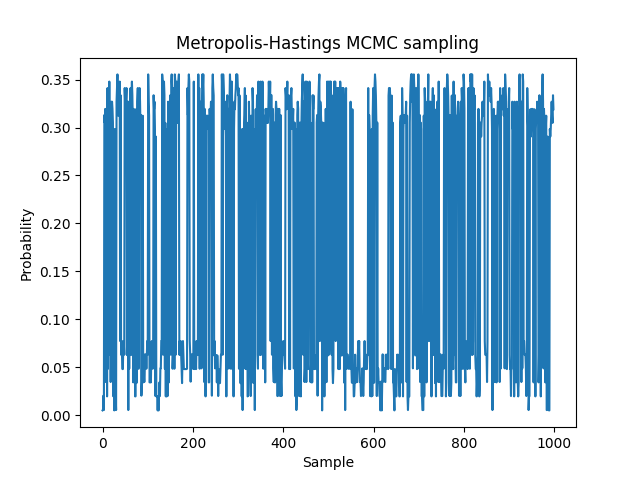
\includegraphics[height=7cm]{task3/V_6_T_6_N_1000.png}
\end{center}
We can observe that the probability distribution provided by the sampling is quite stable.

To understand the accuracy of the method, we compared the true switch settings with the most likely, according to the result. The most likely switch settings are the one that were chosen most often during the sampling. 
\begin{center}
	\begin{tabular}{| c | c | c | c | c | c | c |}
		True $\alpha(\mathbf{v})$ & $R$ & $L$ & $L$ & $R$ & $R$ & $L$ \\
		ML $\alpha(\mathbf{v})$ & $R$ & $L$ & $R$ & $R$ & $R$ & $L$ \\
	\end{tabular}
\end{center}
In particular, we provide the plot of the MCMC Metropolis Hastings label proposals for node 1.
\begin{center}
	\begin{tabular}{| c |}
		$p(\alpha(v_1)=L) = 0.46 $ \\
		$p(\alpha(v_1)=R) = 0.54 $ \\
	\end{tabular}
\end{center}
\begin{center}
	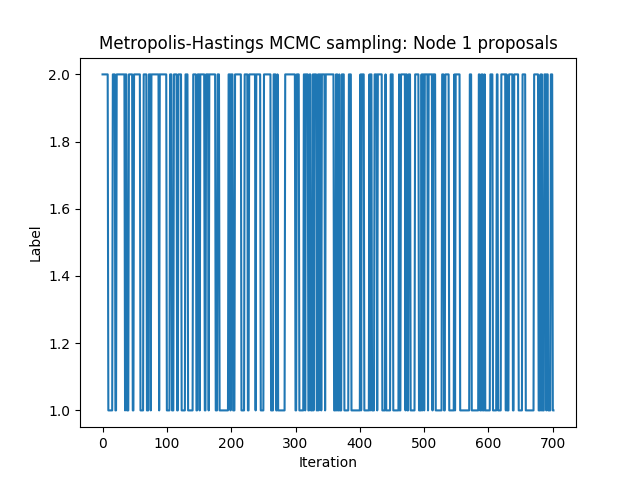
\includegraphics[height=6.8cm]{task3/V_6_T_6_N_1000_Node1.png}
\end{center}
Running again the program, performing $N=10^4$ iterations, we have the following results:
\begin{center}
	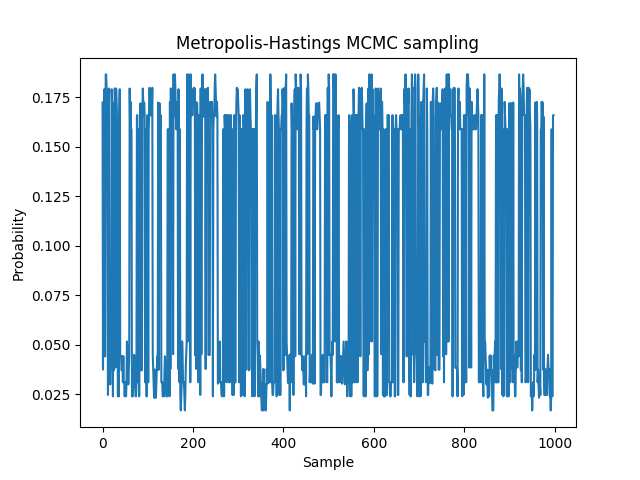
\includegraphics[height=7cm]{task3/V_6_T_6_N_10000.png}
	\begin{tabular}{| c | c | c | c | c | c | c |}
		True $\alpha(\mathbf{v})$ & $R$ & $R$ & $L$ & $L$ & $R$ & $R$ \\
		ML $\alpha(\mathbf{v})$ & $R$ & $R$ & $L$ & $R$ & $R$ & $L$ \\
	\end{tabular}
	\\
	\begin{tabular}{| c |}
		$p(\alpha(v_1)=L) = 0.51 $ \\
		$p(\alpha(v_1)=R) = 0.49 $ \\
	\end{tabular}
\end{center}
Note that in the plots we show just the last $10^3$ iterations to make them more clear to the reader. 

\subsection*{Question 10}
Now, we aim to perform the same analysis using Gibbs sampling instead of Metropolis Hastings. So, at each iteration $i = 1...N$
\begin{enumerate}
	\item[-] sample $\alpha(v_1)$, 
	\item[-] sample $\alpha(v_2)$,
	\item[-] ...
	\item[-] sample $\alpha(v_V)$,  
\end{enumerate} 
In particular, for each node $j \in V(G)$, the sampling step is done according to
$$
\text{with probability } \frac{1}{2} \text{, } \alpha(v_j^{i+1}) = \alpha(v_j^i)
$$
$$
\text{with probability } \frac{1}{2} \text{, } \alpha(v_j^{i+1}) \neq \alpha(v_j^i)
$$
Setting $V=6$, $T=6$ and $N=10^4$, we obtained
\begin{center}
	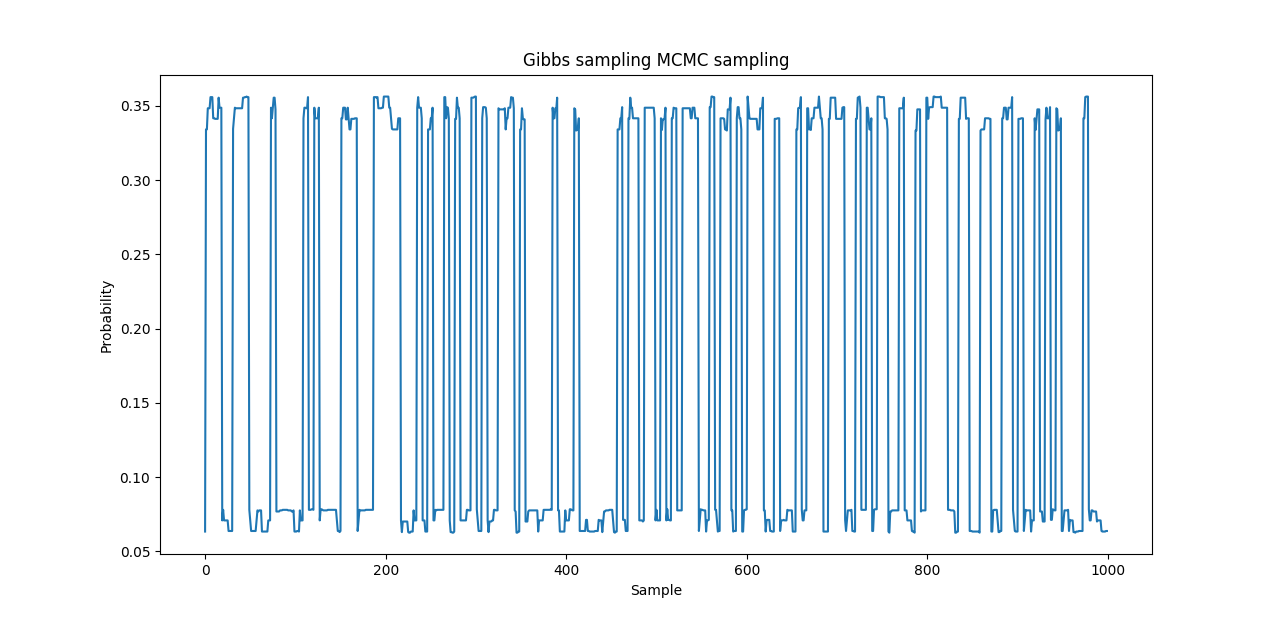
\includegraphics[width=\columnwidth]{task3/V_6_T_6_N_10000_Gibbs.png}
	\begin{tabular}{| c | c | c | c | c | c | c |}
		True $\alpha(\mathbf{v})$ & $R$ & $R$ & $L$ & $L$ & $R$ & $R$ \\
		ML $\alpha(\mathbf{v})$ & $R$ & $R$ & $R$ & $L$ & $L$ & $R$ \\
	\end{tabular}
\end{center}
Considering blocked Gibbs sampling, we can say that the Metropolis Hasting algorithm proposed in the previous part of the task corresponds to blocked Gibbs with blocked size equal to $V$, since in MH we change randomly one component of the switch setting vector at each iteration. We could consider any size for blocked Gibbs: if we consider $n \leq V$ ($n > 1$) groups of components at each iteration, then we change randomly $n$ switch settings of $\alpha(\mathbf{v})$.

For instance, we run the blocked Gibbs sampling for $n=2$ with $V=6$, that means that we consider at each iteration 3 groups of components. We obtained a more accurate result:
\begin{center}
	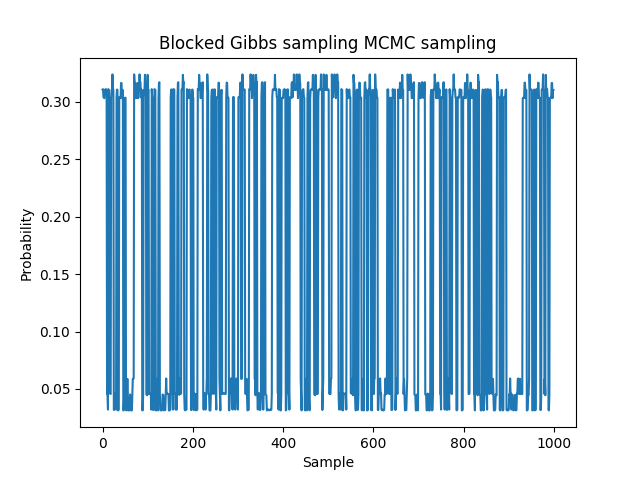
\includegraphics[height=6cm]{task3/V_6_T_6_N_10000_Blocked_Gibbs.png}
	\begin{tabular}{| c | c | c | c | c | c | c |}
		True $\alpha(\mathbf{v})$ & $L$ & $R$ & $L$ & $R$ & $R$ & $R$ \\
		ML $\alpha(\mathbf{v})$ & $L$ & $R$ & $L$ & $R$ & $R$ & $R$ \\
	\end{tabular}
\end{center}

In our sampling algorithms we do not need to sample the stop position $s$ for the reasoning about proposals and acceptance probabilities that we provided at the beginning of the task. However, we could compute the probability associated to each stop position given the switch settings. 

\newpage

\section*{2.5 Stochastic volatility unknown parameter}
Let us consider the problem presented in task 2.1. Now, we assume that the variance parameters $\sigma$ and $\beta$ are both unknown, while $\phi$ is given. The Bayesian setting is characterized by the priors:
$$
\sigma^2 \sim \mathit{IG}(a=0.01, b=0.01)
$$
$$
\beta^2 \sim \mathit{IG}(a=0.01, b=0.01)
$$
Then, we obtain the posterior distributions of the variance parameters in closed form:
$$
p(\sigma^2|\phi, x_{0:T}, y_{1:T}) = \mathit{IG}(\sigma^2|a+\frac{T}{2}, b+\frac{1}{2}\sum_{t=1}^{T}(x_t-\phi x_{t-1})^2)
$$
$$
p(\beta^2|\phi, x_{0:T}, y_{1:T}) = \mathit{IG}(\sigma^2|a+\frac{T}{2}, b+\frac{1}{2}\sum_{t=1}^{T}e^{-x_t}y_t^2)
$$

\subsection*{Question 13}
We implemented a particle Gibbs sampler to compute the posterior distribution $p(\sigma^2, \beta^2|\phi, y_{1:T})$. To do so, at each iteration we alternatively sample from
\begin{enumerate}
	\item[-] $p(\sigma^2|\phi, x_{0:T}, y_{1:t})$
	\item[-] $p(\beta^2|\phi, x_{0:T}, y_{1:t})$
	\item[-] $p(x_{0:T}|\theta, y_{1:T})$
\end{enumerate}
The initialization is perfomed considering, as first value of $\sigma^2$ the true value, i.e., $\sigma = 0.1646$. Then we sample the first values of $x_t$, for $t=0...T$, considering the distributions presented in task 2.1.

Considering $N=10^4$ and $T=500$, we obtained the following marginal distributions:


\end{document}

